\documentclass[a4paper,11pt]{article}
\usepackage{a4wide}

\usepackage{amsmath,latexsym,amssymb}
\usepackage{graphicx}
\graphicspath{ {./figures_final_exam/} }
% Required packages for plotting
\usepackage{pgfplots}
%\usepackage{pgfplotstable}
\pgfplotsset{compat=1.16}
%\usepackage{tikz}
\usepackage{multicol}
\usepackage{logicproof}

% Main document
\begin{document}
\title{Dynamic Epistemic Logic - Final Take Home Exam}
\author{Thomas Pappas}
%\date{}
\maketitle

\section*{Exercise 1}

\paragraph{(a)} Let $F=\left<S,R\right>$ be a frame.

\subparagraph{($\Leftarrow$)} Let $M=\left<S,R,V\right>$ for some $V$ such that the property holds.
Then
\begin{flalign}
	& M,w \models \Box \Box p \rightarrow \Box p \nonumber\\
	\Leftrightarrow & M,w \models \Box \Box p \Rightarrow M,w \models \Box p \nonumber\\
	\Leftrightarrow & (\forall s \in R[w])[M,s \models \Box p] \Rightarrow (\forall s \in R[w])[M,s \models p] \nonumber\\
	\Leftrightarrow & (\forall s \in R[w])\left[(\forall t \in R[s]) [M,t \models p]\right] \Rightarrow (\forall s \in R[w])[M,s \models p] \label{ex1arl}
\end{flalign}
From hypothesis we get that $(\forall s \in R[w])\exists u \in R[w]$ such that $s \in R[u]$ therefore the first part of \eqref{ex1arl} implies that $M,s \models p, \forall s \in R[w]$ and therefore implies the second.
Therefore it holds.

\subparagraph{($\Rightarrow$)} Let $\Box \Box p \rightarrow \Box p$ hold in $F$ and assume $R$ doesn't have the weak density property, i.e. $\exists s,t$ such that $t \in R[s]$ but $\nexists u$ such that $u \in R[s]$ and $t \in R[u]$.
Define $V(p) = R[t], \forall t \in R[s]$ and $V(q) = \emptyset, q \ne p$.
\begin{center}
	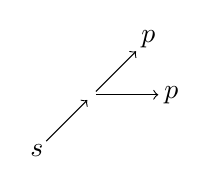
\begin{tikzpicture}[
			shorten >=1pt,
			main/.style = {inner sep=1pt}
		]
		\node[main] (s) {$s$};
		\node[main] (empty1) [above right of=s] {};
		\node[main] (p1) [above right of=empty1] {$p$};
		\node[main] (p2) [right of=empty1] {$p$};
		\draw[->] (s) to (empty1);
		\draw[->] (empty1) to (p1);
		\draw[->] (empty1) to (p2);
	\end{tikzpicture}
\end{center}
Then $M,s \models \Box  \Box p$ but $M,s \not\models \Box p$ which is absurd.

\paragraph{(b)} The formula that defines the property $\forall x \forall y (xRy \rightarrow xRx)$ is
\[\Diamond p \rightarrow (\Box p \rightarrow p)\]
\subparagraph{($\Leftarrow$)} Let $M=\left<S,R,V\right>$ for some $V$ such that the property holds.
Then
\begin{flalign*}
	& M,w \models \Diamond p \rightarrow (\Box p \rightarrow p) \nonumber\\
	\Leftrightarrow & M,w \models \Diamond p  \Rightarrow M,w \models (\Box p \rightarrow p)
\end{flalign*}
From hypothesis, for $w$ if we have $M,w \models \Diamond p$ then $\exists y (y \in R[w])$ and from the property we get that $w$ is reflective, and therefore $M,w \models \Box p \rightarrow p$ also holds.

\subparagraph{($\Rightarrow$)} Let $\Diamond p \rightarrow (\Box p \rightarrow p$ hold in $F$ and assume that $R$ does not have the above property.
Consider the model where $w \notin V(p)$ but $s \in V(p)$ for an $s \in R[w]$
\begin{center}
	\begin{tikzpicture}[
		shorten >=1pt,
		main/.style = {inner sep=1pt}
	]
	\node[main] (w) {$w$};
	\node[main] (p) [above right of=empty1] {$p$};
	\draw[->] (w) to (p);
	\end{tikzpicture}
\end{center}
Then we have $M,w \models \Diamond p, M,w \models \Box p$ but $M,w \not\models p$.
\\[8pt]
Therefore the above modal formula indeed defines the property $\forall x \forall y (xRy \rightarrow xRx)$.


\section*{Exercise 2}

\paragraph{(a)} We see the following cases
\begin{itemize}
	\item If I was holding two aces, then Bob would see 4 aces in total and would figure out he is holding two eights.
		Not true since Bob cannot determine his cards.
	\item If i was holding two eights, then Alice would see 4 eight in total and would figure out she is holding two eights.
		Not true since Alice cannot determine her cards.
\end{itemize}
Therefore I am holding an ace and an eight.

\paragraph{(b)} Since I see two eights from Alice and an ace and an eight from Bob, it means I either have two aces or an ace and an eight.
If I hade two aces, then Bob would be in the same position as myself in (a), and since he still cannot determine his cards it means that is not the case.
Therefore I hold an ace and an eight.

\paragraph{(c)} We see the following cases
\begin{itemize}
	\item If I had two eights, then Alice would be in the same position as myself in (b) and she would have figured out her cards in her second round.
	\item If I had two aces, then the same logic can be applied as in (b) and therefore Alice would again figure out her cards.
\end{itemize}
Therefore I hold an ace and an eight.

\paragraph{(d)} We denote as $A$ when a player holds an ace and $8$ when they hold an eight.
Considering all posible cases for three players, the possible words of the game are
\begin{itemize}
	\item $(AA,AA,88),(AA,88,AA),(88,AA,AA)$
	\item $(AA,88,88),(88,AA,88),(88,88,AA)$
	\item $(AA,A8,A8),(A8,AA,A8),(A8,A8,AA)$
	\item $(88,A8,A8),(A8,88,A8),(A8,A8,88)$
	\item $(AA,A8,88),(AA,88,A8),(A8,AA,88),(A8,88,A8),(88,AA,A8),(88,A8,AA)$
	\item $(A8,A8,A8)$
\end{itemize}

\paragraph{(e)}
\[\] % Added to make the figure show below the paragraph label.
\begin{figure}[h]
	\centering
	\includegraphics[width=1\textwidth]{aces_eights_kripke}
	\caption{The Kripke structure describing the aces and eights game}
\end{figure}

\paragraph{(f)} Considering the situation described in part (a), when Alice and Bob say they cannot determine which cards they have, the structure becomes as such
\begin{figure}[h]
	\centering
	\includegraphics[width=0.5\textwidth]{aces_eights_kripke_f}
	\caption{The Kripke structure after Alice and Bob's turns}
\end{figure}


\section*{Exercise 3}

\subsection*{Exercise 4.20}

We will show that $M,s \models \left<\phi\right> K_a \psi$ iff $M,s \models (\phi \land K_a(\phi \rightarrow \left<\phi\right>\psi))$
\begin{flalign*}
	& M,s \models (\phi \land K_a(\phi \rightarrow \left<\phi\right>\psi))\\
	\Leftrightarrow & M,s \models \phi \text{ and } M,s \models K_a(\phi \rightarrow \left<\phi\right>\psi)\\
	\Leftrightarrow & M,s \models \phi \text{ and } (\forall t \in R[s]) [M,t \models \phi \rightarrow \left<\phi\right>\psi]\\
	\Leftrightarrow & M,s \models \phi \text{ and } (\forall t \in R[s]) [M,t \models \phi \text{ implies } M,t \models \left<\phi\right>\psi]\\
	\Leftrightarrow & M,s \models \phi \text{ and } (\forall t \in R[s]) [M,t \models \phi \text{ implies } (M,t \models \phi \text{ and } M|_\phi,t \models \psi)]\\
	\Leftrightarrow & M,s \models \phi \text{ and } (\forall t \in R[s]) [M,t \models \phi \text{ implies } M|_\phi,t \models \psi]\\
	\Leftrightarrow & M,s \models \phi \text{ and } (\forall t \in R[s]: M,t \models \phi) \text{ implies } M|_\phi,t \models \psi\\
	\Leftrightarrow & M,s \models \phi \text{ and } (\forall t \in R[s]|_\phi) \text{ implies } M|_\phi,t \models \psi\\
	\Leftrightarrow & M,s \models \phi \text{ and } M|_\phi,s \models K_a\psi\\
	\Leftrightarrow & M,s \models \left<\phi\right> K_a\psi
\end{flalign*}

\subsection*{Exercise 4.21}
In Example 4.1 from the book we can first see that the formula $\phi = \left<p \land \neg K_b p\right>\hat{K}_a\hat{K}_b \neg p$ is not valid for the $0$ world since
\[M,0 \not\models p \Rightarrow M,0 \not\models p \land \neg K_b p\]
Then for the $1$ world we have that $M,1 \models p$, but also $M,1 \models \neg K_b p$ since $\neg K_b p \leftrightarrow \hat{K}_b \neg p$ and indeed $b$ considers possible the $0$ world where $\neg p$ holds.
Then we see that $M,1 \models \hat{K}_a\hat{K}_b \neg p$, because
\begin{align*}
	& M,0 \models \neg p \\
	\Rightarrow & M,1 \models \hat{K}_b \neg p & \text{ (since } 0 \sim_b 1 \text{)}\\
	\Rightarrow & M,1 \models \hat{K}_a \hat{K}_b \neg p & \text{ (since } 1 \sim_a 1 \text{)}
\end{align*}
Therefore finally we have
\[M,1 \models p \text{ and } M,1 \models \neg K_b p \text{ and } M,1 \models \hat{K}_a\hat{K}_b \neg p \Rightarrow M,1 \models \left<p \land \neg K_b p\right>\hat{K}_a\hat{K}_b \neg p\]


\section*{Exercise 4}

We will use induction on the formula $\phi$.

\paragraph{if $\phi = p$} then $\phi(p/\psi) = \psi$ and $\phi(p/\chi) = \chi$ and finally $\vdash \psi \leftrightarrow \chi$ from hypothesis

\paragraph{if $\phi = \neg \phi^\prime$} then $\phi(p/\psi) = \neg \phi^\prime(p/\psi)$ and $\phi(p/\chi) = \neg \phi^\prime(p/\chi)$.
So we have
\begin{logicproof}{1}
	\vdash \phi^\prime(p/\psi) \leftrightarrow \phi^\prime(p/\chi) & (induction hypothesis) \\
	\vdash \neg \phi^\prime(p/\psi) \leftrightarrow \neg \phi^\prime(p/\chi) & (1, propositional) \\
	\vdash \phi(p/\psi) \leftrightarrow \phi(p/\chi) &
\end{logicproof}

\paragraph{if $\phi = \phi_1 \land \phi_2$} then $\phi(p/\psi) = \phi_1(p/\psi) \land \phi_2(p/\psi)$ and $\phi(p/\chi) = \phi_1(p/\chi) \land \phi_2(p/\chi)$.\\
So we have
\begin{logicproof}{1}
	\vdash \phi_1(p/\psi) \leftrightarrow \phi_1(p/\chi) & (induction hypothesis) \\
	\vdash \phi_2(p/\psi) \leftrightarrow \phi_2(p/\chi) & (induction hypothesis) \\
	\vdash \phi_1(p/\psi) \land \phi_2(p/\psi) \leftrightarrow \phi_1(p/\chi) \land \phi_2(p/\chi) & (1,2, propositional) \\
	\vdash \phi(p/\psi) \leftrightarrow \phi(p/\chi) &
\end{logicproof}

\paragraph{if $\phi = K_a \phi^\prime$} then $\phi(p/\psi) = K_a \phi^\prime(p/\psi)$ and $\phi(p/\chi) = K_a \phi^\prime(p/\chi)$.\\
So we have
\begin{logicproof}{1}
	\vdash \phi^\prime(p/\psi) \leftrightarrow \phi^\prime(p/\chi) & (induction hypothesis) \\
	\vdash K_a(\phi^\prime(p/\psi) \leftrightarrow \phi^\prime(p/\chi)) & (1, necessitation of $K_a$) \\
	\vdash K_a(\phi^\prime(p/\psi) \rightarrow \phi^\prime(p/\chi)) & (2, propositional) \\
	\vdash K_a(\phi^\prime(p/\psi)) \rightarrow K_a(\phi^\prime(p/\chi)) & (3, distribution of $K_a$ over $\rightarrow$) \\
	\vdash K_a(\phi^\prime(p/\chi) \rightarrow \phi^\prime(p/\psi)) & (2, propositional) \\
	\vdash K_a(\phi^\prime(p/\chi)) \rightarrow K_a(\phi^\prime(p/\psi)) & (5, distribution of $K_a$ over $\rightarrow$) \\
	\vdash K_a(\phi^\prime(p/\psi)) \leftrightarrow K_a(\phi^\prime(p/\chi)) & (4,6, propositional) \\
	\vdash \phi(p/\psi) \leftrightarrow \phi(p/\chi) &
\end{logicproof}

\paragraph{if $\phi = [\phi_1]\phi_2$} then $\phi(p/\psi) = [\phi_1(p/\psi)]\phi_2(p/\psi)$ and $\phi(p/\chi) = [\phi_1(p/\chi)]\phi_2(p/\chi)$.
\\[8pt]
Here we will also use the following tautology (for arbitrary $\phi_1,\phi_2,\psi,\chi$)
\begin{equation}
	((\phi_1 \rightarrow \psi) \land (\phi_2 \rightarrow \chi) \land (\phi_1 \leftrightarrow \phi_2)) \rightarrow (\psi \leftrightarrow \chi) \label{t1}
\end{equation}
So we have
\begin{logicproof}{1}
	\vdash \phi_2(p/\psi) \rightarrow [\phi_1(p/\psi)]\phi_2(p/\psi) & (from $\phi$ follows $[\psi]\phi$) \\
	\vdash \phi_2(p/\chi) \rightarrow [\phi_1(p/\chi)]\phi_2(p/\chi) & (from $\phi$ follows $[\psi]\phi$) \\
	\vdash \phi_2(p/\psi) \leftrightarrow \phi_2(p/\chi) & (inductive hypothesis) \\
	\vdash [\phi_1(p/\psi)]\phi_2(p/\psi) \leftrightarrow [\phi_1(p/\chi)]\phi_2(p/\chi) & (1,2,3, tautology \eqref{t1}, modus ponence) \\
	\vdash \phi(p/\psi) \leftrightarrow \phi(p/\chi) &
\end{logicproof}
\newpage

\section*{Exercise 5}

We have the following models:
\begin{multicols}{2}
	\[M = (\text{Read};\text{Read}_b)=\left<S,\sim,\textbf{pre}\right>\]
	\columnbreak
	\begin{center}
		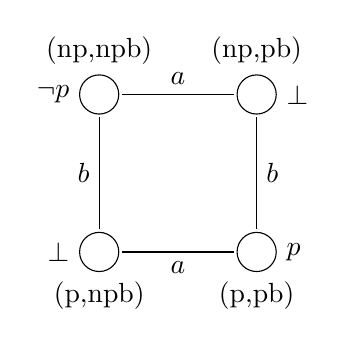
\begin{tikzpicture}[
				node distance={20mm},
				shorten >=1pt,
				shorten <=1pt,
				main/.style = {draw, circle, inner sep=5pt}
			]
			\node[main, label={(np,npb)}, label=left:{$\neg p$}] (nn) {};
			\node[main, label={(np,pb)}, label=right:{$\bot$}] (np) [right of=nn] {};
			\node[main, label=below:{(p,npb)}, label=left:{$\bot$}] (pn) [below of=nn] {};
			\node[main, label=below:{(p,pb)}, label=right:{$p$}] (pp) [right of=pn] {};
			\draw[-] (nn) to node[above] {$a$} (np);
			\draw[-] (nn) to node[left] {$b$} (pn);
			\draw[-] (np) to node[right] {$b$} (pp);
			\draw[-] (pn) to node[below] {$a$} (pp);
		\end{tikzpicture}
	\end{center}
\end{multicols}
\begin{multicols}{2}
	\[M^\prime = (\text{Read};\text{Read}_b)^\prime=\left<S^\prime,\sim^\prime,\textbf{pre}^\prime\right>\]
	\columnbreak
	\begin{center}
		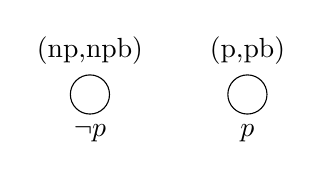
\begin{tikzpicture}[
				node distance={20mm},
				shorten >=1pt,
				shorten <=1pt,
				main/.style = {draw, circle, inner sep=5pt}
			]
			\node[main, label={(np,npb)}, label=below:{$\neg p$}] (nn) {};
			\node[main, label={(p,pb)}, label=below:{$p$}] (pp) [right of=nn] {};
		\end{tikzpicture}
	\end{center}
\end{multicols}
In order to show that $M$ is emulus to $M^\prime$ we will use the definition in footnote 4 from p.159 of the book.
We consider the relation
\[\mathfrak{E} = S \times S^\prime\]
We will show that $\mathfrak{E}$ is an emulation between $(M,(\text{np,npb}))$ and $(M^\prime,(\text{np,npb}))$.
We indeed have $\mathfrak{E}((\text{np,npb}),(\text{np,npb}))$

\paragraph{Front}
\begin{itemize}
	\item For $\mathfrak{E}((\text{np,npb}),(\text{np,npb}))$ and $(\text{np,npb}) \sim_a (\text{np,pb})$ we have\\
		$(\text{np,npb}) \sim^\prime_a (\text{np,npb})$ and $\mathfrak{E}((\text{np,npb}),(\text{np,pb}))$
	\item For $\mathfrak{E}((\text{np,npb}),(\text{np,npb}))$ and $(\text{np,npb}) \sim_b (\text{p,npb})$ we have\\
		$(\text{np,npb}) \sim^\prime_b (\text{np,npb})$ and $\mathfrak{E}((\text{np,npb}),(\text{p,npb}))$
	\item For $\mathfrak{E}((\text{np,pb}),(\text{np,npb}))$ and $(\text{np,pb}) \sim_b (\text{p,pb})$ we have\\
		$(\text{np,pb}) \sim^\prime_b (\text{np,npb})$ and $\mathfrak{E}((\text{np,npb}),(\text{p,pb}))$
	\item For $\mathfrak{E}((\text{p,npb}),(\text{np,npb}))$ and $(\text{p,npb}) \sim_a (\text{p,pb})$ we have\\
		$(\text{p,npb}) \sim^\prime_a (\text{np,npb})$ and $\mathfrak{E}((\text{np,npb}),(\text{p,pb}))$
\end{itemize}

\paragraph{Back}
For each $\text{t}^\prime \in S^\prime$ we only have $\text{t}^\prime \sim^\prime_a \text{t}^\prime$ and $\text{t}^\prime \sim^\prime_b \text{t}^\prime$ so for $\mathfrak{E}(\text{t},\text{t}^\prime)$ we selecting $\text{t}$ again suffices since also $\text{t} \sim_a \text{t}$ and $\text{t} \sim_b \text{t}$

\paragraph{Pre}
For all $\mathfrak{E}(\text{t},(\text{np,npb})), \text{t} \in S$ iy holds that there are $(\text{np,npb}),(\text{p,pb}) \in S^\prime$ where
\[\textbf{pre}(\text{t}) \models \textbf{pre}^\prime(\text{np,npb}) \lor \textbf{pre}^\prime(\text{p,pb}) \Rightarrow \textbf{pre}(\text{t}) \models p \lor \neg p \Rightarrow \textbf{pre}(\text{t}) \models \top\]
which holds for all $\text{t} \in S$. For the reverse we only need to select t and (np,npb) and
\[\textbf{pre}^\prime(\text{np,npb}) \models \text{pre(t)} \lor \textbf{pre}(\text{np,npb}) \Rightarrow \neg p \models \text{pre(t)} \lor \neg p\]
which holds, and therefore $\mathfrak{E}$ is an emulation between $(M,(\text{np,npb}))$ and $(M^\prime,(\text{np,npb}))$.
\\[8pt]
Likewise we can show that $\mathfrak{E}$ is an emulation between $(M,(\text{p,pb}))$ and $(M^\prime,(\text{p,pb}))$ and therefore $\mathfrak{E}$ is a total emulation.


\section*{Exercise 6}

We will use the Example 6.38 of the book where $\vdash_{\textbf{AMC}} [\text{Read, p}]K_a p$.
We also note that using the same logic we get $\vdash_{\textbf{AMC}} [\text{Read, np}]K_a \neg p$.\\
So we have
\begin{footnotesize}
\begin{logicproof}{1}
	\vdash_{\textbf{AMC}} [\text{Read, p}]K_a p & (Example 6.38) \\
	\vdash_{\textbf{AMC}} [\text{Read, p}](K_a p \lor K_a \neg p) & (1, propositional) \\
	\vdash_{\textbf{AMC}} K_b[\text{Read, p}](K_a p \lor K_a \neg p) & (2, necessitation of $K_b$) \\
	\vdash_{\textbf{AMC}} p \rightarrow K_b[\text{Read, p}](K_a p \lor K_a \neg p) & (3, weakening) \\
	\vdash_{\textbf{AMC}} [\text{Read, np}]K_a \neg p & (Example 6.38 for np) \\
	\vdash_{\textbf{AMC}} [\text{Read, np}](K_a p \lor K_a \neg p) & (5, propositional) \\
	\vdash_{\textbf{AMC}} K_b[\text{Read, p}](K_a p \lor K_a \neg p) & (6, necessitation of $K_b$) \\
	\vdash_{\textbf{AMC}} p \rightarrow K_b[\text{Read, p}](K_a p \lor K_a \neg p) & (7, weakening) \\
	\vdash_{\textbf{AMC}} [\text{Read, p}]K_b(K_a p \lor K_a \neg p) \leftrightarrow (p \rightarrow \bigwedge_{\text{s} \sim_b \text{t}} K_b[\text{Read, t}](K_a p \lor K_a \neg p)) & (pre(p) $=p$, action and knowledge) \\
	\vdash_{\textbf{AMC}} [\text{Read, p}]K_b(K_a p \lor K_a \neg p) & ($[\text{p}]_{\sim_b} = \{\text{p,np}\}$, 4,8,9, propositional)
\end{logicproof}
\end{footnotesize}

\end{document}
